\subsection{Outer Measures and Extension Theorems}

\begin{definition} \label{def:abstract-outer-measure-clean-division} \hlt{Abstract Outer Measure and Clean Division}\\
Let $M$ be a set.
\begin{enumerate}[label=(\roman*)]
\setlength{\itemsep}{0pt}
\item An \hlt{abstract outer measure} on $M$ is a map $\omega:2^M\to[0,+\infty]$ such that $\omega(\emptyset)=0$, $A\subseteq B\Rightarrow\omega(A)\leq\omega(B)$, and $\omega(\bigcup_{k=1}^{\infty}A_k)\leq\sum_{k=1}^{\infty}\omega(A_k)$ for all $A,B,A_k\subseteq M$.
\item For an outer measure $\omega$, $E\subseteq M$ is \hlt{$\omega$-measurable} iff $\omega(X)=\omega(X\cap E)+\omega(X\cap E^c)$ for every $X\subseteq M$.
\end{enumerate}
For $\omega=m_n^\ast$, $\omega$-measurability is Caratheodory measurability.
\end{definition}

\begin{definition} \label{def:cover-induced-outer-measure} \hlt{Outer Measure Induced by a Covering Family}\\
Let $\mathcal{S}\subseteq\mathcal{P}(X)$ and let $\rho:\mathcal{S}\to[0,+\infty]$.
\begin{enumerate}[label=(\roman*)]
\setlength{\itemsep}{0pt}
\item For $E\subseteq X$, $\mathcal{C}_{\mathcal{S}}(E)\defeq\{(S_k)_{k\geq1}\in\mathcal{S}^{\N}:E\subseteq\bigcup\limits_{k=1}^{\infty}S_k\}$.
\item The induced map $\rho^\ast:\mathcal{P}(X)\to[0,+\infty]$ is defined by $\rho^\ast(\emptyset)=0$ and,\\
for $E\neq\emptyset$, $\rho^\ast(E)\defeq\inf\limits_{(S_k)\in\mathcal{C}_{\mathcal{S}}(E)}\sum\limits_{k=1}^{\infty}\rho(S_k)$, with $\inf\emptyset=+\infty$.
\end{enumerate}
The map $\rho^\ast$ is the \hlt{outer measure induced by $\rho$ and $\mathcal{S}$}.\\
\hlt{Key Insight}: Minimize total $\rho$-cost over countable $\mathcal{S}$-covers.
\end{definition}

\begin{proposition} \label{prop:cover-induced-set-function-is-outer-measure} \hlt{Cover-Induced Outer Measure}\\
For $\mathcal{S}\subseteq\mathcal{P}(X)$ and $\rho:\mathcal{S}\to[0,+\infty]$, the cover-induced map $\rho^\ast:\mathcal{P}(X)\to[0,+\infty]$ is an outer measure on $X$.
\begin{proof} By construction, $\rho^\ast(\emptyset)=0$ and $\rho^\ast\geq0$. If $A\subseteq B$, then $\mathcal{C}_{\mathcal{S}}(B)\subseteq\mathcal{C}_{\mathcal{S}}(A)$, hence $\rho^\ast(A)\leq\rho^\ast(B)$.\\
Let $E=\bigcup\limits_kE_k$, $I=\{k:E_k\neq\emptyset\}$, and assume $I\neq\emptyset$ and $\sum\limits_k\rho^\ast(E_k)<+\infty$.\\
Choose $(S_{k,j})_j\in\mathcal{C}_{\mathcal{S}}(E_k)$ for $k\in I$ with $\sum\limits_j\rho(S_{k,j})<\rho^\ast(E_k)+\varepsilon2^{-k}$.\\
Since $(S_{k,j})_{k\in I,j\geq1}$ covers $E$, $\rho^\ast(E)\leq\sum\limits_{k\in I}\sum\limits_j\rho(S_{k,j})\leq\sum\limits_k\rho^\ast(E_k)+\varepsilon$; let $\varepsilon\downarrow0$. Excluded cases are immediate.\\
\hlt{Structural Commentary}: Inclusion orders covers; regrouping covers sums.\\
\hlt{Key Insight}: Covers generate subadditivity.
\end{proof}
\end{proposition}

\begin{lemma} \label{lem:caratheodory-finite-measure-test} \hlt{Finite-Measure Test for Caratheodory Measurability}\\
Let $\omega:2^M\to[0,+\infty]$ be an outer measure. Then $E\subseteq M$ is $\omega$-measurable iff, for all $X\subseteq M$,\\
$\omega(X)<+\infty\Longrightarrow \omega(X)\geq\omega(X\cap E)+\omega(X\cap E^c)$.
\begin{proof}
\begin{enumerate}[label=\roman*.]
\setlength{\itemsep}{0pt}
\item[$(\Rightarrow)$] If $E$ is $\omega$-measurable, then $\omega(X)=\omega(X\cap E)+\omega(X\cap E^c)$ $\forall X\subseteq M$, hence finite-test inequality holds.
\item[$(\Leftarrow)$] For all $X\subseteq M$, $X=(X\cap E)\sqcup(X\cap E^c)$ gives $\omega(X)\leq\omega(X\cap E)+\omega(X\cap E^c)$. If $\omega(X)<+\infty$, the hypothesis gives $\geq$; if $\omega(X)=+\infty$, $\geq$ is automatic in $[0,+\infty]$. Thus equality holds for every $X$.
\end{enumerate}
\hlt{Structural Commentary}: To verify a clean split, only finite outer-measure test sets need real work.\\
\hlt{Key Insight}: Subadditivity supplies one inequality for free.
\end{proof}
\end{lemma}

\begin{figure}[H]
  \centering
  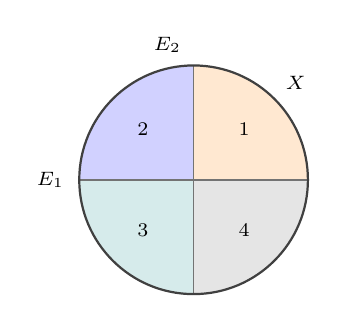
\begin{tikzpicture}[
  scale=0.88,
  every node/.style={font=\scriptsize},
  cut/.style={black!55, line width=0.65pt},
  boundary/.style={black!75, line width=0.8pt}
]
  \begin{scope}
    \clip (0,0) circle (1.65);
    \fill[orange!18] (0,0) rectangle (1.65,1.65);
    \fill[blue!18] (-1.65,0) rectangle (0,1.65);
    \fill[teal!16] (-1.65,-1.65) rectangle (0,0);
    \fill[black!10] (0,-1.65) rectangle (1.65,0);
    \draw[cut] (-1.65,0) -- (1.65,0);
    \draw[cut] (0,-1.65) -- (0,1.65);
  \end{scope}

  \draw[boundary] (0,0) circle (1.65);

  \node at (0.73,0.73) {$1$};
  \node at (-0.73,0.73) {$2$};
  \node at (-0.73,-0.73) {$3$};
  \node at (0.73,-0.73) {$4$};

  \node[above left=1pt] at (0,1.65) {$E_2$};
  \node[left=2pt] at (-1.65,0) {$E_1$};
  \node[above right=1pt] at (1.15,1.12) {$X$};
\end{tikzpicture}

  \caption{Two cuts split $X$ into four regions; $E_1\setminus E_2$ is region $2$.}
  \label{fig:measurable-difference-four-regions}
\end{figure}

\begin{definition} \label{def:outer-measure-zero-sets} \hlt{Zero Sets}\\
For outer measure $\omega:2^M\to[0,+\infty]$, \hlt{$\omega$-zero set} is $Z\subseteq M$ with $\omega(Z)=0$; $\mathcal{Z}_\omega\defeq\{Z\subseteq M:\omega(Z)=0\}$.
\end{definition}

\begin{theorem} \label{thm:caratheodory-measurable-sets-sigma-algebra} \hlt{Caratheodory Measurable Sets}\\
Let $\omega:2^M\to[0,+\infty]$ be an outer measure.\\
Let $\mathcal{M}_\omega\defeq\{E\subseteq M:\omega(X)=\omega(X\cap E)+\omega(X\cap E^c)\ \forall X\subseteq M\}$ and $\mathcal{Z}_\omega\defeq\{Z\subseteq M:\omega(Z)=0\}$. Then:
\begin{enumerate}[label=(\roman*)]
\setlength{\itemsep}{0pt}
\item $\mathcal{Z}_\omega\subseteq\mathcal{M}_\omega$;
\item $\mathcal{M}_\omega$ is a $\sigma$-algebra;
\item $\omega|_{\mathcal{M}_\omega}$ is countably additive;
\item if $E\in\mathcal{M}_\omega$ and $Z\in\mathcal{Z}_\omega$, then $E\cup Z,E\setminus Z,E\triangle Z\in\mathcal{M}_\omega$ and $\omega(E\cup Z)=\omega(E\setminus Z)=\omega(E\triangle Z)=\omega(E)$.
\end{enumerate}
\begin{proof}
\begin{enumerate}[label=(\roman*)]
\setlength{\itemsep}{0pt}
\item If $Z\in\mathcal{Z}_\omega$ and $X\subseteq M$, then $\omega(X)\leq\omega(X\cap Z)+\omega(X\cap Z^c)\leq0+\omega(X)$, so equality holds and $Z\in\mathcal{M}_\omega$.
\item Complements are immediate. If $E,F\in\mathcal{M}_\omega$, with $E^1=E$, $E^0=E^c$, $F^1=F$, and $F^0=F^c$, then $\omega(X)=\sum_{\epsilon,\eta\in\{0,1\}}\omega(X\cap E^\epsilon\cap F^\eta)$; hence finite Boolean combinations are measurable.\\
For pairwise disjoint $E_i\in\mathcal{M}_\omega$, set $E=\bigsqcup_iE_i$ and $F_N=(\bigcup_{i=1}^{N}E_i)^c$.\\
Finite splitting gives $\omega(X)\geq\sum_{i=1}^{N}\omega(X\cap E_i)+\omega(X\cap E^c)$ for every $N$.\\
Letting $N\to\infty$ and using subadditivity gives $\omega(X)=\sum_{i=1}^{\infty}\omega(X\cap E_i)+\omega(X\cap E^c)$.\\
Since $\omega(X\cap E)\leq\sum_i\omega(X\cap E_i)$ and $\omega(X)\leq\omega(X\cap E)+\omega(X\cap E^c)$, $E\in\mathcal{M}_\omega$.\\
General countable unions follow from $H_1=E_1$ and $H_n=E_n\setminus\bigcup_{i<n}E_i$.
\item If $E=\bigsqcup_{i=1}^{\infty}E_i$ with $E_i\in\mathcal{M}_\omega$, then the equality in (ii) with $X=E$ gives $\omega(E)=\sum_{i=1}^{\infty}\omega(E_i)$.
\item By (i)--(ii), $E\cup Z,E\setminus Z,E\triangle Z\in\mathcal{M}_\omega$.\\
Since $E\cap Z$ and $Z\setminus E$ are null, additivity gives $\omega(E\setminus Z)=\omega(E\cup Z)=\omega(E\triangle Z)=\omega(E)$.
\end{enumerate}
\hlt{Structural Commentary}: Measurable sets preserve countable additivity.\\
\hlt{Key Insight}: Measurable cuts turn subadditivity into equality.
\end{proof}
\end{theorem}

\begin{corollary} \label{cor:caratheodory-disjointization-countable-additivity} \hlt{Disjointization of Countable Measurable Unions}\\
Let $\omega:2^M\to[0,+\infty]$ be an outer measure and let $(E_k)_{k\geq1}\subseteq\mathcal{M}_\omega$.\\
Set $F_1\defeq E_1$ and $F_k\defeq E_k\setminus\bigcup\limits_{i=1}^{k-1}E_i$ for $k\geq2$.\\
Then $(F_k)$ is pairwise disjoint in $\mathcal{M}_\omega$, $\bigcup\limits_{k\geq1}F_k=\bigcup\limits_{k\geq1}E_k$, and $\omega(\bigcup\limits_{k\geq1}E_k)=\sum\limits_{k\geq1}\omega(F_k)$ in $[0,+\infty]$.
\begin{proof}
Since $\mathcal{M}_\omega$ is a $\sigma$-algebra, $F_k=E_k\cap(\bigcup\limits_{i<k}E_i)^c\in\mathcal{M}_\omega$. If $i<k$, then $F_i\cap F_k\subseteq E_i\cap(\bigcup\limits_{j<k}E_j)^c=\emptyset$.\\
For $x\in\bigcup\limits_{k\geq1}E_k$, $x\in F_{\min\{j:x\in E_j\}}$; hence $\bigcup\limits_{k\geq1}F_k=\bigcup\limits_{k\geq1}E_k$, and countable additivity gives $\omega(\bigcup\limits_{k\geq1}E_k)=\sum\limits_{k\geq1}\omega(F_k)$.\\
\hlt{Structural Commentary}: Disjointization turns unions into sums.\\
\hlt{Key Insight}: Peel off earlier pieces so a countable union becomes a disjoint sum.
\end{proof}
\end{corollary}

\begin{definition} \label{def:sigma-and-sigma-delta-cover-classes} \hlt{Countable Cover Classes}\\
Let $\mathcal{S}\subseteq\mathcal{P}(X)$.
\begin{enumerate}[label=(\roman*)]
\setlength{\itemsep}{0pt}
\item \hlt{Countable-union class}: $\mathcal{S}_\sigma\defeq\left\{\bigcup\limits_{n=1}^{\infty}S_n:(S_n)_{n\geq1}\in\mathcal{S}^{\N}\right\}$.
\item \hlt{Countable-intersection class}: $\mathcal{S}_{\sigma\delta}\defeq\left\{\bigcap\limits_{n=1}^{\infty}A_n:(A_n)_{n\geq1}\in(\mathcal{S}_\sigma)^{\N}\right\}$.
\end{enumerate}
\hlt{Key Insight}: $\mathcal{S}_\sigma$ closes under countable unions; $\mathcal{S}_{\sigma\delta}$ then closes once under countable intersections.
\end{definition}

\begin{proposition} \label{prop:finite-outer-measure-sigma-delta-envelope} \hlt{Finite Outer-Measure Envelope}\\
Let $\mathcal{S}\subseteq\mathcal{P}(X)$, let $\rho:\mathcal{S}\to[0,+\infty]$, and let $\rho^\ast$ be the cover-induced map.\\
If $\emptyset\neq E\subseteq X$ and $\rho^\ast(E)<+\infty$, then there exists $A\in\mathcal{S}_{\sigma\delta}$ such that:
\begin{enumerate}[label=(\roman*)]
\setlength{\itemsep}{0pt}
\item $E\subseteq A$ and $\rho^\ast(A)=\rho^\ast(E)$.
\item If $E$ and every $S\in\mathcal{S}$ are $\rho^\ast$-measurable, then $A$ is $\rho^\ast$-measurable and $\rho^\ast(A\setminus E)=0$.
\end{enumerate}
\begin{proof} $\forall n\geq1$, choose $(S_{n,k})_{k\geq1}\in\mathcal{C}_{\mathcal{S}}(E)$ with $\sum\limits_{k=1}^{\infty}\rho(S_{n,k})<\rho^\ast(E)+\frac{1}{n}$. Set $A_n\defeq\bigcup\limits_{k=1}^{\infty}S_{n,k}$, $A\defeq\bigcap\limits_{n=1}^{\infty}A_n$.\\
Then $A_n\in\mathcal{S}_\sigma$, $A\in\mathcal{S}_{\sigma\delta}$, $E\subseteq A\subseteq A_n$, and $\rho^\ast(A_n)<\rho^\ast(E)+\frac{1}{n}$.
\begin{enumerate}[label=(\roman*)]
\setlength{\itemsep}{0pt}
\item Monotonicity gives $\rho^\ast(E)\leq\rho^\ast(A)\leq\rho^\ast(A_n)<\rho^\ast(E)+\frac{1}{n}$ for all $n$, hence $\rho^\ast(A)=\rho^\ast(E)$.
\item If $E$ and every $S\in\mathcal{S}$ are $\rho^\ast$-measurable, then the $\rho^\ast$-measurable sets form a $\sigma$-algebra, so $A_n$ and $A$ are $\rho^\ast$-measurable. Since $E\subseteq A$ and $\rho^\ast(E)<+\infty$, excision gives $\rho^\ast(A\setminus E)=\rho^\ast(A)-\rho^\ast(E)=0$.
\end{enumerate}
\hlt{Structural Commentary}: Finite cost gives a countable-intersection envelope.\\
\hlt{Key Insight}: Cover within $\frac{1}{n}$, then intersect.
\end{proof}
\end{proposition}

\begin{definition} \label{def:outer-measure-generated-by-premeasure} \hlt{Outer Measure Generated by a Premeasure}\\
Let $\mu:\mathcal{A}\to[0,+\infty]$ be a premeasure on an algebra $\mathcal{A}\subseteq\mathcal{P}(X)$.
\begin{enumerate}[label=(\roman*)]
\setlength{\itemsep}{0pt}
\item \hlt{Algebra covers}: For $B\subseteq X$, set $\mathcal{C}_{\mathcal{A}}(B)\defeq\{(E_j)_{j\geq1}\in\mathcal{A}^{\N}:B\subseteq\bigcup\limits_{j=1}^{\infty}E_j\}$.
\item \hlt{Generated outer measure}: Define $\mu^\ast:\mathcal{P}(X)\to[0,+\infty]$ by $\mu^\ast(\emptyset)=0$ and, for $B\neq\emptyset$, $\mu^\ast(B)\defeq\inf\limits_{(E_j)\in\mathcal{C}_{\mathcal{A}}(B)}\sum\limits_{j=1}^{\infty}\mu(E_j)$, with $\inf\emptyset=+\infty$.
\end{enumerate}
\hlt{Key Insight}: Cover arbitrary sets by algebra sets and minimize total premeasure.
\end{definition}

\begin{lemma} \label{lem:generated-outer-measure-basic-properties} \hlt{Generated Outer-Measure Properties}\\
Let $\mu:\mathcal{A}\to[0,+\infty]$ be a premeasure on an algebra $\mathcal{A}\subseteq\mathcal{P}(X)$.\\
For $B\subseteq X$, put $\mathcal{C}_{\mathcal{A}}(B)\defeq\{(E_j)\in\mathcal{A}^{\N}:B\subseteq\bigcup\limits_jE_j\}$.\\
Set $\inf\emptyset=+\infty$, $\mu^\ast(\emptyset)=0$, and $\mu^\ast(B)\defeq\inf\limits_{(E_j)\in\mathcal{C}_{\mathcal{A}}(B)}\sum\limits_j\mu(E_j)$ for $B\neq\emptyset$. Then:
\begin{enumerate}[label=(\roman*)]
\setlength{\itemsep}{0pt}
\item $\mu^\ast(\emptyset)=0$.
\item If $C\subseteq D\subseteq X$, then $\mu^\ast(C)\leq\mu^\ast(D)$.
\item If $(B_n)_{n\geq1}\subseteq\mathcal{P}(X)$, then $\mu^\ast(\bigcup\limits_{n=1}^{\infty}B_n)\leq\sum\limits_{n=1}^{\infty}\mu^\ast(B_n)$.
\item If $E\in\mathcal{A}$, then $\mu^\ast(E)=\mu(E)$.
\end{enumerate}
\begin{proof}
\begin{enumerate}[label=(\roman*)]
\setlength{\itemsep}{0pt}
\item This is the assigned value of $\mu^\ast(\emptyset)$.
\item If $C\subseteq D$, then $\mathcal{C}_{\mathcal{A}}(D)\subseteq\mathcal{C}_{\mathcal{A}}(C)$; taking infima gives $\mu^\ast(C)\leq\mu^\ast(D)$.
\item Let $B=\bigcup\limits_nB_n$ and $I=\{n:B_n\neq\emptyset\}$. If $I=\emptyset$ or $\sum\limits_n\mu^\ast(B_n)=+\infty$, the claim is immediate.\\
Otherwise, for $\varepsilon>0$ choose $(E_{n,k})_{k\geq1}\in\mathcal{C}_{\mathcal{A}}(B_n)$ for $n\in I$ with $\sum\limits_k\mu(E_{n,k})<\mu^\ast(B_n)+\varepsilon2^{-n}$.\\
Then $(E_{n,k})_{n\in I,k\geq1}$ covers $B$, so $\mu^\ast(B)\leq\sum\limits_{n\in I}\sum\limits_k\mu(E_{n,k})\leq\sum\limits_n\mu^\ast(B_n)+\varepsilon$; let $\varepsilon\downarrow0$.
\item Cover $E,\emptyset,\emptyset,\ldots$ gives $\mu^\ast(E)\leq\mu(E)$. Conversely, for any cover $(F_n)\in\mathcal{C}_{\mathcal{A}}(E)$, set $G_n\defeq E\cap\left(F_n\setminus\bigcup\limits_{k<n}F_k\right)$.\\
Then $(G_n)$ is disjoint in $\mathcal{A}$, $\bigcup\limits_nG_n=E$, and $G_n\subseteq F_n$, so $\mu(E)=\sum\limits_n\mu(G_n)\leq\sum\limits_n\mu(F_n)$.\\
Taking infima gives $\mu(E)\leq\mu^\ast(E)$.
\end{enumerate}
\hlt{Structural Commentary}: Cover containment and regrouping give the outer-measure axioms.\\
\hlt{Key Insight}: Disjointize algebra covers to recover $\mu$.
\end{proof}
\end{lemma}

\begin{proposition} \label{prop:single-set-envelope-vs-generated-outer-measure} \hlt{Single-Set Envelope Comparison}\\
Let $\mu:\mathcal{A}\to[0,+\infty]$ be a premeasure on an algebra $\mathcal{A}\subseteq\mathcal{P}(X)$, let $\mu^\ast$ be the generated outer measure, and define $\mu^\sharp:\mathcal{P}(X)\to[0,+\infty]$ by $\mu^\sharp(B)\defeq\inf\{\mu(C):C\in\mathcal{A},\ B\subseteq C\}$ with $\inf\emptyset=+\infty$.
\begin{enumerate}[label=(\roman*)]
\setlength{\itemsep}{0pt}
\item $\mu^\sharp(E)=\mu(E)$ for every $E\in\mathcal{A}$.
\item $\mu^\ast(B)\leq\mu^\sharp(B)$ for every $B\subseteq X$.
\end{enumerate}
\begin{proof}
\begin{enumerate}[label=(\roman*)]
\setlength{\itemsep}{0pt}
\item If $E\in\mathcal{A}$, then $E$ is admissible, so $\mu^\sharp(E)\leq\mu(E)$.\\
Conversely, $E\subseteq C\in\mathcal{A}$ implies $\mu(E)\leq\mu(C)$ by monotonicity of $\mu$, hence $\mu(E)\leq\mu^\sharp(E)$.
\item If no $C\in\mathcal{A}$ contains $B$, then $\mu^\sharp(B)=+\infty$. Otherwise, each $C\in\mathcal{A}$ with $B\subseteq C$ gives the algebra cover $C,\emptyset,\emptyset,\ldots$, so $\mu^\ast(B)\leq\mu(C)$. Taking infima over such $C$ gives $\mu^\ast(B)\leq\mu^\sharp(B)$.
\end{enumerate}
\hlt{Structural Commentary}: One algebra superset is a special countable cover.\\
\hlt{Key Insight}: The single-set envelope is larger.
\end{proof}
\end{proposition}

\begin{example} \label{ex:single-set-envelope-not-outer-measure} \hlt{Single-Set Envelopes Need Not Be Outer Measures}\\
Let $X$ be uncountable, let $\mathcal{A}$ be the finite--cofinite algebra on $X$, and set $\mu(E)\defeq0$ for finite $E$, $\mu(E)\defeq+\infty$ for cofinite $E$. Then $\mu$ is a premeasure, $\mu^\ast(B)=0$ iff $B$ is countable, and $\mu^\sharp(B)=0$ iff $B$ is finite.\\
For any countably infinite $S\subseteq X$, $\mu^\sharp(S)=+\infty$ while $S=\bigcup_{x\in S}\{x\}$ and $\sum_{x\in S}\mu^\sharp(\{x\})=0$, QED.\\
\hlt{Structural Commentary}: Countable covers can be strictly smaller than one-set covers.\\
\hlt{Key Insight}: Outer measure is built from countable covers precisely to recover countable subadditivity.
\end{example}

\begin{theorem} \label{thm:generated-caratheodory-extension} \hlt{Generated Caratheodory Extension}\\
Let $\mu:\mathcal{A}\to[0,+\infty]$ be a premeasure on an algebra $\mathcal{A}\subseteq\mathcal{P}(X)$. For $B\subseteq X$, put\\
$\mathcal{C}_{\mathcal{A}}(B)\defeq\{(E_j)\in\mathcal{A}^{\N}:B\subseteq\bigcup\limits_jE_j\}$. Define $\mu^\ast(\emptyset)=0$, $\mu^\ast(B)\defeq\inf\limits_{(E_j)\in\mathcal{C}_{\mathcal{A}}(B)}\sum\limits_j\mu(E_j)$ for $B\neq\emptyset$ with $\inf\emptyset=+\infty$, and $\mathcal{C}_\mu\defeq\{E\subseteq X:(\forall B\subseteq X)\ \mu^\ast(B)=\mu^\ast(B\cap E)+\mu^\ast(B\setminus E)\}$. Then:
\begin{enumerate}[label=(\roman*)]
\setlength{\itemsep}{0pt}
\item $\mathcal{A}\subseteq\mathcal{C}_\mu$ and $\mu^\ast|_{\mathcal{A}}=\mu$.
\item $\mathcal{C}_\mu$ is a $\sigma$-algebra on $X$.
\item $\mu^\ast|_{\mathcal{C}_\mu}$ is a complete measure extending $\mu$.
\end{enumerate}
\begin{proof}
Lemma \ref{lem:generated-outer-measure-basic-properties} makes $\mu^\ast$ an outer measure and gives $\mu^\ast|_{\mathcal{A}}=\mu$.
\begin{enumerate}[label=(\roman*)]
\setlength{\itemsep}{0pt}
\item Let $E\in\mathcal{A}$ and $B\subseteq X$. Subadditivity gives $\mu^\ast(B)\leq\mu^\ast(B\cap E)+\mu^\ast(B\setminus E)$. If $(F_n)\in\mathcal{C}_{\mathcal{A}}(B)$, then $F_n\cap E,F_n\setminus E\in\mathcal{A}$ and $\mu(F_n)=\mu(F_n\cap E)+\mu(F_n\setminus E)$, so $\mu^\ast(B\cap E)+\mu^\ast(B\setminus E)\leq\sum\limits_n\mu(F_n)$.\\
Infimizing over $(F_n)$ gives equality; hence $E\in\mathcal{C}_\mu$. The lemma gives $\mu^\ast|_{\mathcal{A}}=\mu$.
\item The class $\mathcal{C}_\mu$ is exactly the $\mu^\ast$-measurable class $\mathcal{M}_{\mu^\ast}$.\\
Since $\mu^\ast$ is an outer measure, Theorem \ref{thm:caratheodory-measurable-sets-sigma-algebra}(ii) gives that $\mathcal{C}_\mu$ is a $\sigma$-algebra on $X$.
\item Theorem \ref{thm:caratheodory-measurable-sets-sigma-algebra}(iii) gives countable additivity of $\mu^\ast|_{\mathcal{C}_\mu}$. If $A\subseteq Z\in\mathcal{C}_\mu$ and $\mu^\ast(Z)=0$, then monotonicity gives $\mu^\ast(A)=0$, so Theorem \ref{thm:caratheodory-measurable-sets-sigma-algebra}(i) gives $A\in\mathcal{C}_\mu$. Thus $\mu^\ast|_{\mathcal{C}_\mu}$ is complete, and (i) shows it extends $\mu$.
\end{enumerate}
\hlt{Structural Commentary}: Caratheodory equality is the additivity domain.\\
\hlt{Key Insight}: Algebra sets split every algebra cover.
\end{proof}
\end{theorem}

\begin{proposition} \label{prop:caratheodory-splitters-finite-subadditive-size} \hlt{Caratheodory Splitters for Finitely Subadditive Size}\\
Let $\alpha:\mathcal{P}(X)\to[0,+\infty)$ satisfy $0\leq\alpha(E)\leq\alpha(E\cup F)\leq\alpha(E)+\alpha(F)$ for all $E,F\subseteq X$.\\
Set $\mathcal{S}\defeq\{E\subseteq X:(\forall A\subseteq X)\ \alpha(A)=\alpha(A\cap E)+\alpha(A\setminus E)\}$.
\begin{enumerate}[label=(\roman*)]
\setlength{\itemsep}{0pt}
\item If $\mathcal{S}\neq\emptyset$, then $\mathcal{S}$ is an algebra on $X$.
\item If $E,F\in\mathcal{S}$ and $E\cap F=\emptyset$, then $\alpha(E\cup F)=\alpha(E)+\alpha(F)$.
\item The hypothesis $\mathcal{S}\neq\emptyset$ in (i) is necessary: if $\alpha\equiv1$, then $\mathcal{S}=\emptyset$.
\end{enumerate}
\begin{proof}
\begin{enumerate}[label=(\roman*)]
\setlength{\itemsep}{0pt}
\item Choose $E_0\in\mathcal{S}$. Splitting $\emptyset$ gives $\alpha(\emptyset)=0$, hence $\emptyset,X\in\mathcal{S}$.\\
Complement symmetry gives $E\in\mathcal{S}\Rightarrow X\setminus E\in\mathcal{S}$. For $E,F\in\mathcal{S}$ and $A\subseteq X$, put $A_{11}=A\cap E\cap F$, $A_{10}=A\cap E\setminus F$, $A_{01}=A\cap F\setminus E$, and $A_{00}=A\setminus(E\cup F)$. By successive splitting,\\
$\alpha(A)=\alpha(A_{11})+\alpha(A_{10})+\alpha(A_{01})+\alpha(A_{00})$; $\alpha(A\setminus(E\cap F))=\alpha(A_{10})+\alpha(A_{01})+\alpha(A_{00})$.\\
Thus $\alpha(A)=\alpha(A\cap E\cap F)+\alpha(A\setminus(E\cap F))$, so $E\cap F\in\mathcal{S}$. Complements give finite unions.
\item Since $F\subseteq X\setminus E$, the splitting identity for $E$ applied to $A=E\cup F$ gives $\alpha(E\cup F)=\alpha(E)+\alpha(F)$.
\item If $\alpha\equiv1$ and $E\in\mathcal{S}$, applying the splitting identity to $A=\emptyset$ gives $1=1+1$, impossible.
\end{enumerate}
\hlt{Structural Commentary}: Splitters are Boolean once one splitter exists.\\
\hlt{Key Insight}: Empty-set splitting forces $\alpha(\emptyset)=0$.
\end{proof}
\end{proposition}

\begin{theorem} \label{thm:sigma-finite-generated-extension-uniqueness} \hlt{$\sigma$-Finite Generated Extensions Are Unique}\\
Let $\mu:\mathcal{A}\to[0,+\infty]$ be a premeasure on an algebra $\mathcal{A}\subseteq\mathcal{P}(X)$, let $\mu^\ast$ be generated by $\mu$, and put\\
$\mathcal{C}_\mu\defeq\{E\subseteq X:(\forall B\subseteq X)\ \mu^\ast(B)=\mu^\ast(B\cap E)+\mu^\ast(B\setminus E)\}$. Assume $X=\bigcup\limits_nF_n$; $F_n\in\mathcal{A}$, $\mu(F_n)<+\infty$ $\forall n$.
\begin{enumerate}[label=(\roman*)]
\setlength{\itemsep}{0pt}
\item $\mu^\ast|_{\mathcal{C}_\mu}$ is a measure on $\mathcal{C}_\mu$ and extends $\mu$.
\item If $\nu$ is a measure on $\mathcal{C}_\mu$ with $\nu|_{\mathcal{A}}=\mu$, then $\nu=\mu^\ast|_{\mathcal{C}_\mu}$.
\end{enumerate}
\begin{proof}
\begin{enumerate}[label=(\roman*)]
\setlength{\itemsep}{0pt}
\item By Theorem \ref{thm:generated-caratheodory-extension}, $\mathcal{C}_\mu$ is complete $\sigma$-algebra, $\mathcal{A}\subseteq\mathcal{C}_\mu$, $\mu^\ast|_{\mathcal{C}_\mu}$ is complete measure with $(\mu^\ast|_{\mathcal{C}_\mu})|_{\mathcal{A}}=\mu$.
\item Let $\nu$ be a measure on $\mathcal{C}_\mu$ with $\nu|_{\mathcal{A}}=\mu$.\\
If $G\in\mathcal{C}_\mu$ and $G\subseteq\bigcup\limits_nA_n$ with $A_n\in\mathcal{A}$, then $\nu(G)\leq\sum\limits_n\mu(A_n)$; hence $\nu(G)\leq\mu^\ast(G)$.\\
If $\mu(X)<+\infty$, apply to $G=E$, $G=X\setminus E$, while $\nu(E)+\nu(X\setminus E)=\nu(X)=\mu^\ast(X)=\mu^\ast(E)+\mu^\ast(X\setminus E)$, gives $\nu(E)=\mu^\ast(E)$. In general, put $H_N\defeq\bigcup\limits_{j=1}^{N}F_j$. Then $H_N\in\mathcal{A}$ and $\mu(H_N)<+\infty$. Apply bound to\\
$E\cap H_N$, $H_N\setminus E$, while $\nu(E\cap H_N)+\nu(H_N\setminus E)=\nu(H_N)=\mu^\ast(H_N)=\mu^\ast(E\cap H_N)+\mu^\ast(H_N\setminus E)$, gives $\nu(E\cap H_N)=\mu^\ast(E\cap H_N)$. Since $E\cap H_N\uparrow E$, continuity from below gives $\nu(E)=\mu^\ast(E)$.
\end{enumerate}
\hlt{Structural Commentary}: Finite uniqueness localizes along a finite-mass exhaustion.\\
\hlt{Key Insight}: Compare on each finite piece, then pass upward.
\end{proof}
\end{theorem}

\begin{corollary} \label{cor:sigma-finite-premeasure-unique-on-generated-sigma-algebra} \hlt{Uniqueness on the Generated $\sigma$-Algebra}\\
Let $\mu:\mathcal{A}\to[0,+\infty]$ be a premeasure on an algebra $\mathcal{A}\subseteq\mathcal{P}(X)$, and assume $X=\bigcup\limits_nF_n$ with $F_n\in\mathcal{A}$ and $\mu(F_n)<+\infty$. If measures $\nu_1,\nu_2$ on $\sigma(\mathcal{A})$ extend $\mu$, then $\nu_1=\nu_2$.
\begin{proof} Put $H_n\defeq\bigcup\limits_{j=1}^{n}F_j$. Then $H_n\in\mathcal{A}$, $H_n\uparrow X$, and $\nu_i(H_n)=\mu(H_n)<+\infty$.\\
For fixed $n$, $\mathcal{D}_n\defeq\{E\in\sigma(\mathcal{A}):\nu_1(E\cap H_n)=\nu_2(E\cap H_n)\}$ is a Dynkin class by finite mass on $H_n$ and contains $\mathcal{A}$, since $A\cap H_n\in\mathcal{A}$. As $\mathcal{A}$ is a $\pi$-system, the $\pi$-$\lambda$ theorem gives $\mathcal{D}_n=\sigma(\mathcal{A})$.\\
Hence $\nu_1(E\cap H_n)=\nu_2(E\cap H_n)$ for all $n$; since $E\cap H_n\uparrow E$, continuity from below gives $\nu_1(E)=\nu_2(E)$.\\
\hlt{Structural Commentary}: Finite exhaustions reduce uniqueness to Dynkin closure.\\
\hlt{Key Insight}: Compare on $H_n$, then pass upward.
\end{proof}
\end{corollary}

\begin{example} \label{ex:rational-half-open-algebra-sigma-finiteness-necessary} \hlt{Why $\sigma$-Finiteness Matters}\\
Let $X=\Q\cap(0,1]$, and let $\mathcal{A}$ be the algebra of finite unions of sets $(a,b]\cap X$, where $0\leq a<b\leq1$ and $a,b\in\Q$.
\begin{enumerate}[label=(\roman*)]
\setlength{\itemsep}{0pt}
\item \hlt{Infinite algebra pieces}: Every nonempty $A\in\mathcal{A}$ is infinite.
\item \hlt{Generated $\sigma$-algebra}: For $r\in X$, choose $a_n\in\Q\cap[0,r)$ with $a_n\uparrow r$.\\
Then $\{r\}=\bigcap\limits_{n=1}^{\infty}((a_n,r]\cap X)\in\sigma(\mathcal{A})$, hence $\sigma(\mathcal{A})=\mathcal{P}(X)$.
\item \hlt{Nonunique extensions}: Let $\mu_1$ be counting measure and $\mu_2=2\mu_1$ on $\mathcal{P}(X)$.\\
Since every nonempty $A\in\mathcal{A}$ is infinite, $\mu_1|_{\mathcal{A}}=\mu_2|_{\mathcal{A}}$, but $\mu_1(\{r\})=1\neq2=\mu_2(\{r\})$ for $r\in X$.
\end{enumerate}
Thus uniqueness may fail without $\sigma$-finiteness.\\
\hlt{Key Insight}: Infinite algebra pieces cannot determine singleton scale.
\end{example}
